\chapter{Background}
\label{background}

In this chapter, we give a brief overview of different \gls{AI} techniques that have been considered for implementing the agent for Quoridor in this thesis including the Minimax algorithm, \gls{MCTS} and A-star algorithm.

\subsection{Minimax algorithm} \label{sec:minimax}
Minimax algorithm, first proven by John von Neumann in 1928 in his paper \textit{Zur Theorie Der Gesellschaftsspiele} \citep{v1928theorie}, is a very popular algorithm employed in many decision-making scenarios for e.g., in decision theory, game theory and even philosophy. As suggested by the name minimax, the idea of the algorithm is to minimize the player's loss when the opponent makes a decision that gives the player the maximum loss. This algorithm has been implemented in many multi-player strategy games such as Tic-Tac-Toe \citep{savelli2008tic}. 


Mathematically, a minimax algorithm can be defined by the following equation:
\begin{equation}\label{eq:mmax}
    \bar{v}_i = \min_{a_{-i}} \max_{a_{i}} v_i (a_i, a_{-i})
\end{equation}
where,
\begin{subequations}
\begin{align}
    &i, -i = \text{index of the player of interest, opponent respectively} \\
    &a_i, a_{-i}= \text{action of the player of interest, opponent respectively} \\
    &v_i = \text{value function of player i} \\
    &\bar{v}_i = \text{minimax value of the player of interest}
\end{align}
\end{subequations}

As defined in the Equation \eqref{eq:mmax}, the minimax algorithm comprises of two parts. The first part is maximizing part where the player chooses an action from a set of possible actions to maximize the evaluation of the game. Then, the player determines the subsequent action of the opponent to minimize the evaluation of the game. This is clarified further with the following example.

\begin{figure}
    \centering
    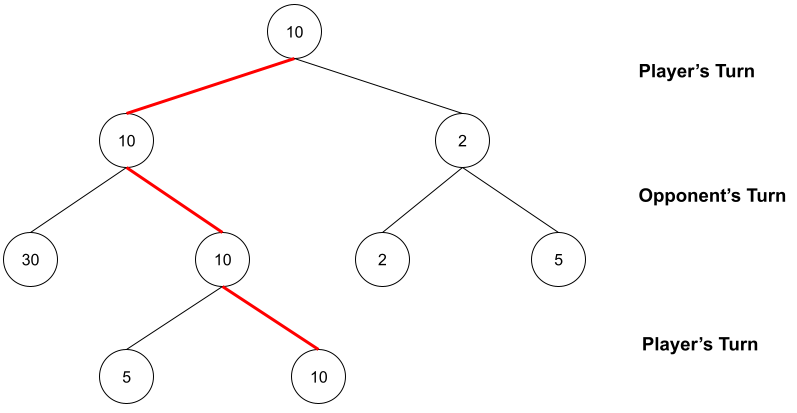
\includegraphics[width=\linewidth]{../img/Minimax1.png}
    \caption{Figure illustrating an exemplary game tree and decision based on minimax algorithm}
    \label{fig:minimax1}
\end{figure}

The Figure \ref{fig:minimax1} consists of nodes that define either player's or the opponent's actions. In our minimax implementation, we have considered an evaluation function as a linear combination of multiple features such as shortest distance to the goal and remaining number of walls. This is explained in detail in Section \ref{sec:gameimplementation}. The numbers for each node Figure \ref{fig:minimax1} represent the evaluation of this function. For each action, there can be an evaluation where higher evaluation may mean it is favouring the player. For example, an action of the player causing two possible evaluations of 10 and 20 would mean the player would have higher advantage choosing the action leading to evaluation of 20. 

The minimax algorithm starts with a game tree with possible moves of the player and opponent. The evaluation of the leaf nodes positions are assigned, for example 5 and 10 in the figure. The player chooses a move to maximize the evaluation on their turn whereas the opponent wants to minimize the evaluation. The player chooses evaluation of 10 (between 10 and 5) on its turn and subsequently evaluation of 10 (between 10 and 30) in the opponent's turn. The red line shows the path the player determines as optimal leading to a decision choosing the the action labelled with evaluation of 10.

The minimax algorithm involves in the player performing an exhaustive search on the game tree to determine a sequence of maximizing and minimizing moves. The complexity of such algorithm in large game tree often means such search is often impossible due to limited computational resources. To limit this complexity, further techniques such as depth-limited minimax, alpha-beta pruning and parallel minimax algorithm can be used.

\subsubsection{Alpha-beta pruning}

\begin{figure}[!ht]
    \centering
    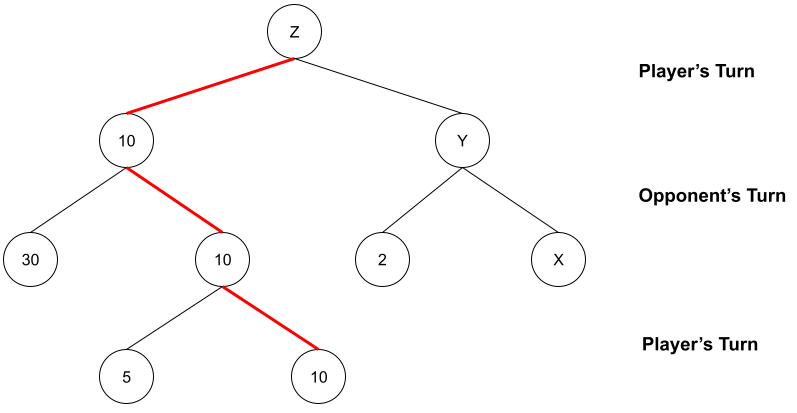
\includegraphics[width=\linewidth]{../img/Minimax2.png}
    \caption{Exemplary figure illustrating the alpha beta pruing for minimax algorithm}
    \label{fig:minimax2}
\end{figure}

Alpha-beta pruning is one way to reduce the compelxity of the minimax algorithm without affecting the performance of it.

In many cases, there may be the actions of the player in the search tree that can be evaluated worse than another action already evaluated. In such cases, where the better move or action has already been determined, it may not be useful to further evaluate the subsequent moves of the player and the opponent. Hence, the alpha-beta pruning reduces the game complexity by not further evaluating the branches of the node with evaluation worse than what has already been determined with another node.

As its name suggests, the alpha beta algorithm maintains two values, alpha and beta values. The alpha value stores the minimum score the player is assured to get while the beta value records the maximum score the opponent is assured to get. Whenever the evaluation of the minimum score of the player is higher than the maximum score after the subsequent move of the opponent (or in other words alpha $>$ beta), the alpha-beta pruning algorithm stops evaluating the opponents position. This reduces the number of nodes in the search tree and hence reduces the complexity of the minimax algorithm.

In Figure \ref{fig:minimax2}, if the player determines that 
\begin{equation}
    Z = max (10, Y) = max (10,  min (2, X)),
\end{equation}
the value of X does not influence the value of $Y$ or $Z$ as $Y = min(2, X) \leq 2$ and hence $Z = max(10, \leq 2) = 10$. In this case, the player may not evaluate the branch $X$ or branch $Y$ further reducing the game tree and hence the computational complexity of the algorithm. 

\subsubsection{Parallel minimax}
Another way to improve the time complexity of the minimax algorithm is to parallelize the algorithm. The minimax algorithm involves in evaluating multiple nodes of the game tree. The way to parallelize such algorithm is to run different processes, in this case, evaluation of the position associated with different nodes, in different threads. This ensures that even though computational complexity may remain the same, the time complexity of the algorithm is distributed over multiple threads and possibly multiple processors.


\subsection{Monte-Carlo Tree Search}\label{sec:MCTS}
\gls{MCTS} \citep{Coulom2006Efficient} is a heuristic tree search algorithm popular in decision-making processes, mostly popular in strategic games where the game tree space is too large to traverse. One problem with the minimax algorithm is that it requires a robust and accurate evaluation function to evaluate a given position in the game. This problem can be even more relevant when the game tree space is too large making it difficult to find the evaluation of a position. The basic idea of the \gls{MCTS} algorithm is that is narrows down on certain areas of the game tree, such that the exhaustive traversal and search of the tree is not required. The algorithm achieves this by taking random samples in the tree space and building a search tree based on it.

\begin{figure}[!ht]
    \centering
    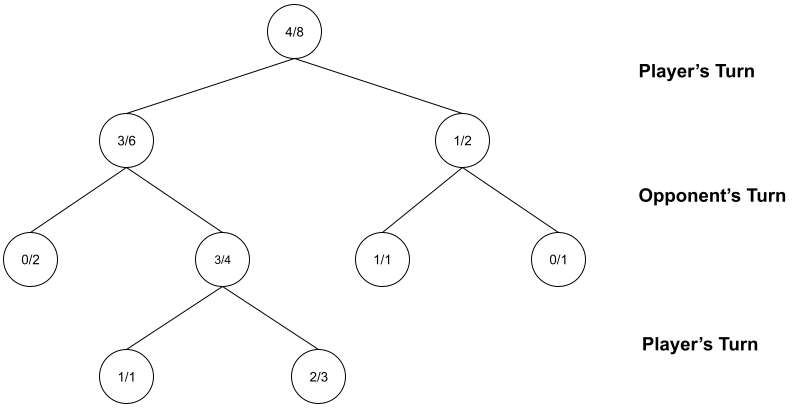
\includegraphics[width = \linewidth]{../img/MCTS1.png}
    \caption{Figure illustrating an iteration of the MCTS algorithm}
    \label{fig:MCTS1}
\end{figure}

As shown in Figure \ref{fig:MCTS1}, \gls{MCTS} algorithm determines the best path to the destination node in the game tree based on multiple trial runs through the game tree. In the figure, each node is labelled with a fraction where the denominator represents the total number of game runs through the node and the numerator represents the total number of wins for the player. For example, the game is simulated a total of 8 times in the example where the player wins 4 of the runs. The player wins 3/6 when taking an action while 1/2 when taking another action and so on.

The \gls{MCTS} algorithm builds upon the following framework:
\begin{enumerate}
    \item \textbf{Selection:} This step involves the algorithm choosing a move based on either a good move determined in previous iterations or a exploratory new move. The algorithm uses the Upper Confidence Bound for Trees \textbf{(UCT)} to guide this decision, balancing the tradeoff between exploration of uncharted nodes and exploitation of nodes with a high success rate.
    
    Mathematically,
    \begin{equation}
        UCT(n) = \overline{X}(n) + c U(n)
    \label{eq:UCT}
    \end{equation}
    where,
    \begin{subequations}
    \begin{align}
        \overline{X}(n) = \text{average win rate of node n} \\
        U(n) = \sqrt{\frac{\ln{N(P(n))}}{N(n)}   }
    \end{align}
    \end{subequations}
    
    
    \item \textbf{Expansion:} This step involves the algorithm to add a new node to the game tree determined during the selection process. A node can simply be a valid move starting from the node from where no simulation step has been played out. In Figure \ref{fig:MCTS2}, an un-evaluated option (e.g., node inside the dotted box) is explored and simulated.
    \item \textbf{Simulation:} This step involves the agent playing out the game using policy. One of the policies can simply be a random policy (e.g., choosing a move based on certain distribution).
    \item \textbf{Back propagation:} Finally, based on the simulation step, this step involves in the algorithm updating the nodes. In Figure \ref{fig:MCTS2}, the red arrows show the back propagation step as a result of exploration and simulation step where the probabilities or the weights of the nodes are updated as a result of exploration and simulation steps.
\end{enumerate}

\begin{figure}[!ht]
    \centering
    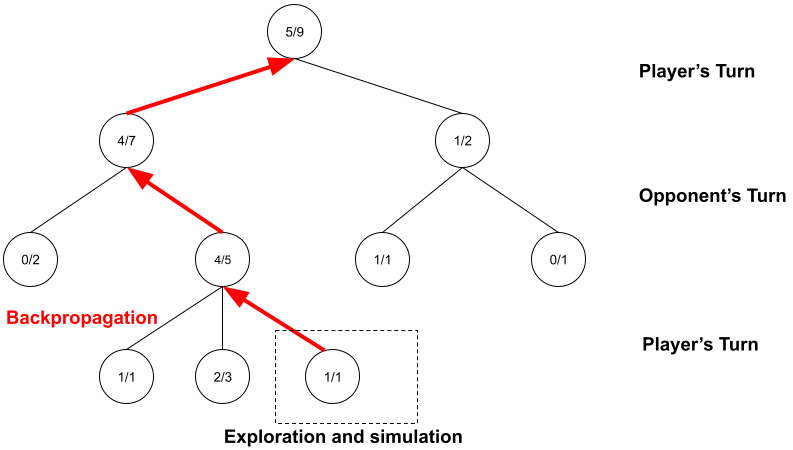
\includegraphics[width=\linewidth]{../img/MCTS2.png}
    \caption{Figure illustrating steps 2, 3, and 4 of the MCTS algorithm}
    \label{fig:MCTS2}
\end{figure}

The advantage of \gls{MCTS} algorithm over the minimax algorithm is that the \gls{MCTS} algorithm does not require any evaluation function as the weights are determined based on multiple simulation runs. On the contrary, the \gls{MCTS} algorithm requires multiple runs through the game to determine the weights.





\subsection{A-star algorithm}
A star is a popular algorithm \citep{Hart1968AFormal} used mainly for graph search and traversal problems. The main aim of the A-star algorithm is to find a path between a starting node and an destination node with the least cost. The cost function of the algorithm comprises of two components, the distance from the starting node to the current node and the estimated heuristic from the current node to the destination node. As the distance to the destination node may not be exactly known, one may use the estimate such as Manhattan distance and Euclidean distance. In the context of Quoridor gameplay, for example, we use the \textit{Manhattan} heuristic (see Equations \ref{eq:playerPHeuristic} and \ref{eq:playerQHeuristic}).

The cost function, or "f" score, for a node depends on two components "g" value and "h" value. "g" value represents the distance from the source node to the node and "h" value represents the cost of the path from the node to the destination node, often defined by a heuristic. Mathematically,
\begin{equation}
    f = g + h
\end{equation}